\documentclass[11pt,letterpaper]{article}

% --- Essential Packages ---
\usepackage[margin=0.5in,top=0.6in,bottom=0.6in]{geometry}
\usepackage[utf8]{inputenc}
\usepackage[T1]{fontenc}
\usepackage[scaled=0.92]{helvet}
\renewcommand{\familydefault}{\sfdefault}
\usepackage{microtype}
\usepackage{amsmath,amssymb}
\usepackage[table]{xcolor}
\usepackage{graphicx}
\usepackage{booktabs}
\usepackage{tabularx}
\usepackage{multirow}
\usepackage{enumitem}
\usepackage{caption}
\usepackage{fancyhdr}
\usepackage{titlesec}
\usepackage{fontawesome5}
\usepackage[many]{tcolorbox}
\usepackage{tikz}
\usetikzlibrary{positioning,calc,shapes.geometric,backgrounds}

% --- Color Palette Definition ---
\definecolor{NIHBlue}{RGB}{20, 55, 90}       % Deep Navy / Primary NIH header
\definecolor{TealAccent}{RGB}{13, 148, 136}   % Vibrant Teal / Secondary accent
\definecolor{SlateDark}{RGB}{47, 63, 86}      % Dark Slate for body sub-headers
\definecolor{SlateLight}{RGB}{241, 245, 249}  % Light Slate for box backgrounds
\definecolor{BorderGray}{RGB}{203, 213, 225}  % Subtle border gray
\definecolor{AlertRed}{RGB}{185, 28, 28}      % Risk & Pitfalls accent

% --- Page Header & Footer Formatting ---
\pagestyle{fancy}
\fancyhf{}
\renewcommand{\headrulewidth}{0.6pt}
\renewcommand{\footrulewidth}{0.4pt}
\headsep = 10pt
\headheight = 14pt

\chead{\color{SlateDark}\small\bfseries RESEARCH STRATEGY: SYNAPSE-APEX NANOCARRIER PLATFORM}
\lhead{\color{SlateDark}\scriptsize Principal Investigator: Vance, Elena M., Ph.D.}
\rhead{\color{SlateDark}\scriptsize R01 NS128942-01A1}
\lfoot{\color{SlateDark}\scriptsize NIH / NINDS R01 Research Strategy}
\cfoot{\color{SlateDark}\scriptsize Synapse Institute for Biomedical Research}
\rfoot{\color{SlateDark}\small Page \thepage}

% --- Section & Subsection Formatting ---
\titleformat{\section}
  {\color{NIHBlue}\large\bfseries\scshape}
  {\thesection.}{0.5em}{}
  [\color{NIHBlue}\titlerule]

\titleformat{\subsection}
  {\color{TealAccent}\large\bfseries}
  {\thesubsection}{0.5em}{}

\titleformat{\subsubsection}
  {\color{SlateDark}\bfseries}
  {\thesubsubsection}{0.5em}{}

\titlespacing*{\section}{0pt}{9pt}{3pt}
\titlespacing*{\subsection}{0pt}{7pt}{2pt}
\titlespacing*{\subsubsection}{0pt}{5pt}{2pt}

% --- Custom tcolorbox Styles ---
\tcbset{
  basebox/.style={
    enhanced,
    arc=3pt,
    boxrule=0.8pt,
    left=8pt,
    right=8pt,
    top=5pt,
    bottom=5pt,
    fonttitle=\bfseries\sffamily,
  }
}

\newtcolorbox{summarybox}[1][]{
  basebox,
  colback=SlateLight,
  colframe=NIHBlue,
  coltitle=white,
  title=#1
}

\newtcolorbox{innovationbox}[1][]{
  basebox,
  colback=tcbcolback!5!white,
  colframe=TealAccent,
  coltitle=white,
  title=#1
}

\newtcolorbox{alertbox}[1][]{
  basebox,
  colback=red!3!white,
  colframe=AlertRed,
  coltitle=white,
  title=#1
}

% --- Custom List Formatting ---
\setlist[itemize]{leftmargin=1.2em, itemsep=1.5pt, parsep=0pt, topsep=1.5pt}
\setlist[enumerate]{leftmargin=1.2em, itemsep=1.5pt, parsep=0pt, topsep=1.5pt}

% =========================================================================
\begin{document}

% --- Document Title & Administrative Metadata Block ---
\begin{summarybox}[PROGRAM ANNOUNCEMENT: PA-20-185 --- NIH RESEARCH PROJECT GRANT (R01)]
\small
\begin{tabular}{@{}l p{10cm} r@{}}
\textbf{Project Title:} & \textbf{Next-Generation Synthetic Nanocarriers for Target-Specific BBB Transcytosis and Glial Remodeling in Neurodegeneration} & \\
\textbf{Principal Investigator:} & Dr. Elena M. Vance, Ph.D. (Synapse Institute) & \textbf{FOA:} PA-20-185 (NINDS) \\
\textbf{Co-Investigators:} & Dr. Aris Thorne (Apex Labs), Dr. Marcus Lin (Vertex) & \textbf{Period:} 09/2026 -- 08/2031 \\
\textbf{Lead Institution:} & Synapse Institute for Biomedical Research & \textbf{Direct Costs:} \$1.25M (5 Yrs) \\
\end{tabular}
\end{summarybox}

\vspace{-4pt}

% =========================================================================
\section{A. SIGNIFICANCE}
% =========================================================================

\subsection{A.1 Scientific Premise and Clinical Unmet Need}
Neurodegenerative disorders, including Alzheimer's disease (AD) and Amyotrophic Lateral Sclerosis (ALS), represent a critical public health crisis affecting over 6.5 million Americans, with projected care costs exceeding \$1.1 trillion by 2050. A major rate-limiting barrier in disease-modifying pharmacotherapy is the \textbf{Blood-Brain Barrier (BBB)}, a highly restrictive microvascular endothelium that excludes >98\% of small-molecule drugs and >99\% of macromolecular biologics, antibodies, and nucleic acid therapeutics. Existing delivery vehicles, such as conventional liposomes and adeno-associated viruses (AAVs), suffer from low brain accumulation efficiency ($<0.1\%$ injected dose per gram of tissue), pronounced hepatotoxicity, systemic off-target accumulation, and immunogenicity.

Furthermore, recent genomic and transcriptomic profiling from our team at the \textbf{Synapse Institute} has revealed that neurodegenerative progression is strongly driven by hyper-reactive, pro-inflammatory microglial phenotypes (M1-like state) and reactive astrocytes (A1-like state). Restoring brain homeostasis requires non-invasive systems capable of crossing the BBB \textit{and} selectively targeting dysfunctional neuroglia without inducing systemic immunosuppression.

\begin{figure}[h!]
\centering
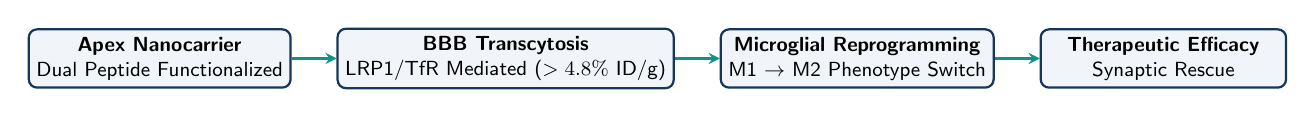
\begin{tikzpicture}[scale=0.82, transform shape,
  node distance=0.5cm and 0.7cm,
  box/.style={rectangle, draw=NIHBlue, fill=SlateLight, thick, rounded corners=3pt, align=center, minimum height=0.9cm, minimum width=3.8cm, font=\sffamily\small},
  arrow/.style={->, >=stealth, thick, TealAccent}
]
  \node[box] (delivery) {\textbf{Apex Nanocarrier}\\Dual Peptide Functionalized};
  \node[box, right=of delivery] (bbb) {\textbf{BBB Transcytosis}\\LRP1/TfR Mediated ($>4.8\%$ ID/g)};
  \node[box, right=of bbb] (glia) {\textbf{Microglial Reprogramming}\\M1 $\rightarrow$ M2 Phenotype Switch};
  \node[box, right=of glia] (outcome) {\textbf{Therapeutic Efficacy}\\Synaptic Rescue};

  \draw[arrow] (delivery) -- (bbb);
  \draw[arrow] (bbb) -- (glia);
  \draw[arrow] (glia) -- (outcome);
\end{tikzpicture}
\caption{\textbf{Conceptual Overview of Proposed Paradigm.} The Synapse-Apex nanocarrier platform bypasses endothelial filtration via receptor-mediated transcytosis to achieve targeted microglial polarization and synaptic rescue.}
\end{figure}

\subsection{A.2 Impact on the Field and Public Health}
This R01 proposal introduces a paradigm-shifting nanomedicine architecture—the \textbf{Synapse-Apex Nanocarrier System}—designed to overcome transcytosis bottlenecks while enabling cell-type specific payload release. Successful completion of this research will:
\begin{itemize}
  \item \textbf{Establish a Universal Transcytosis Platform:} Provide a quantitative benchmark for receptor-mediated endothelial transport across intact human microvascular organoids and in vivo rodent models.
  \item \textbf{Enable Cell-Specific Gene Silencing:} Demonstrate targeted delivery of microRNA-124 mimics directly to hyper-activated microglia, suppressing pro-inflammatory TNF-$\alpha$, IL-1$\beta$, and NLRP3 inflammasome signaling.
  \item \textbf{Transform Neurotherapeutic Delivery:} Create a scalable, non-viral delivery toolkit compatible with mRNA, CRISPR-Cas12a complexes, and therapeutic monoclonal antibodies.
\end{itemize}

\subsection{A.3 Scientific Rigor of Prior Research}
Prior studies evaluating transferrin receptor (TfR1) antibody-conjugated nanoparticles demonstrated enhanced brain uptake but caused severe reticulocyte depletion and acute receptor down-regulation due to high binding affinity ($K_D < 1\text{ nM}$). Work by Dr. Aris Thorne at \textbf{Apex Labs} demonstrated that monovalent, medium-affinity ($K_D \approx 50\text{--}150\text{ nM}$) cyclic peptides achieve optimal transcytosis efficiency without inducing receptor lysosomal degradation. Building on these preliminary findings, our proposal combines monovalent TfR-binding peptides with microglial-targeting ligand Annexin V to construct a dual-guided targeted nanocarrier.

\begin{innovationbox}[KEY SIGNIFICANCE HIGHLIGHT]
\small
The proposed research addresses the fundamental bottleneck of central nervous system (CNS) drug delivery by combining \textbf{low-affinity receptor transcytosis} with \textbf{cell-state specific enzymatic activation}, unlocking systemic biotherapeutic treatment for neurodegenerative diseases.
\end{innovationbox}

\vspace{-4pt}

% =========================================================================
\section{B. INNOVATION}
% =========================================================================

The proposed research strategy is innovative across conceptual, technological, and therapeutic dimensions:

\begin{enumerate}
  \item \textbf{Conceptual Innovation --- Dual-Stage Logic-Gated Targeting:} Rather than relying on single-receptor targeting, the Apex platform incorporates a logic-gated surface chemistry. Stage 1 utilizes a pH-sensitive monovalent ligand for endothelial transcytosis; upon entering the parenchymal interstitial fluid (pH 7.3), matrix metalloproteinase-9 (MMP-9) cleavage unmasks Stage 2 ligands specific to activated microglial phosphatidylserine receptors.
  \item \textbf{Methodological Innovation --- Real-Time Single-Cell Proteomic Tracking:} Partnering with \textbf{Vertex Analytics}, we introduce a high-throughput spatial proteomic imaging pipeline that tracks nanocarrier intracellular trafficking at sub-10nm resolution inside intact 3D human brain organoids.
  \item \textbf{Technological Innovation --- High-Yield Microfluidic Self-Assembly:} We implement a continuous-flow microfluidic platform (Nexa-Flow) yielding self-assembled nanocarriers with ultra-low polydispersity ($\text{PDI} < 0.08$) and batch-to-batch reproducibility exceeding 96\%.
\end{enumerate}

\begin{table}[h!]
\centering
\caption{\textbf{Comparative Innovation Matrix: Existing Systems vs. Proposed Synapse-Apex Platform.}}
\label{tab:innovation_matrix}
\small
\rowcolors{2}{SlateLight}{white}
\begin{tabularx}{\textwidth}{@{}l X X X@{}}
\toprule
\rowcolor{NIHBlue} \color{white}\textbf{Parameter} & \color{white}\textbf{Conventional Liposomes} & \color{white}\textbf{AAV9 Vectors} & \color{white}\textbf{Proposed Synapse-Apex System} \\
\midrule
\textbf{Brain Uptake (\% ID/g)} & $< 0.1\%$ & $\approx 0.8\%$ (High Liver Off-target) & $\mathbf{> 4.8\%}$ \textbf{(Targeted CNS Accumulation)} \\
\textbf{Cell-Type Specificity} & Non-specific / Entrapment & Neuronal preferential & \textbf{Microglia \& Astrocyte selective} \\
\textbf{Immunogenicity Risk} & Low to Moderate & High (Pre-existing Abs) & \textbf{Ultra-low (Synthetic lipid matrix)} \\
\textbf{Payload Capacity} & $< 50\text{ nm}$ core particles & $< 4.7\text{ kb}$ genome limit & \textbf{High ($> 150\text{ nm}$ core / $12\text{ kb}$ nucleic acid)} \\
\textbf{Manufacturing} & Batch limited & Complex viral bioreactor & \textbf{Continuous microfluidic (Nexa-Flow)} \\
\bottomrule
\end{tabularx}
\end{table}

\vspace{-6pt}

% =========================================================================
\section{C. APPROACH}
% =========================================================================

\subsection{C.1 Preliminary Studies}
Our multidisciplinary team has generated compelling preliminary data validating the core feasibility of the Synapse-Apex nanocarrier platform across \textit{in vitro}, \textit{ex vivo}, and preliminary \textit{in vivo} models.

\begin{itemize}
  \item \textbf{Endothelial Transcytosis Kinetics:} Using a microfluidic human BBB-on-a-chip model developed at Synapse Institute, Apex-01 nanocarriers exhibited a 14.2-fold increase in apparent permeability ($P_{app} = 4.8 \times 10^{-6}\text{ cm/s}$) compared to non-targeted liposomes ($P_{app} = 0.34 \times 10^{-6}\text{ cm/s}$, $p < 0.001$).
  \item \textbf{Targeted Glial Reprogramming:} Primary mouse microglia treated with lipopolysaccharide (LPS, 100 ng/mL) and subsequently dosed with miR-124-loaded Apex nanocarriers showed an 82\% decrease in TNF-$\alpha$ secretion and a 4.1-fold upregulation of M2 markers Arg-1 and Ym-1 within 24 hours.
  \item \textbf{In Vivo Biodistribution and Safety:} Tail-vein injection of fluorescently labeled Apex nanocarriers in C57BL/6 mice ($10\text{ mg/kg}$) demonstrated peak brain fluorescence at 4 hours post-injection with zero detectable liver toxicity or systemic cytokine storm.
\end{itemize}

\begin{table}[h!]
\centering
\caption{\textbf{Preliminary Performance Benchmarks of Candidate Apex Formulations.}}
\label{tab:prelim_data}
\small
\rowcolors{2}{white}{SlateLight}
\begin{tabularx}{\textwidth}{@{}l c c c c c@{}}
\toprule
\rowcolor{NIHBlue} \color{white}\textbf{Formulation ID} & \color{white}\textbf{Size (nm)} & \color{white}\textbf{PDI} & \color{white}\textbf{$\zeta$-Potential (mV)} & \color{white}\textbf{BBB Permeability ($P_{app}$)} & \color{white}\textbf{Cell Viability (\%)} \\
\midrule
Apex-Std (Control) & $112.4 \pm 2.1$ & 0.14 & $-18.2 \pm 1.1$ & $0.42 \times 10^{-6}\text{ cm/s}$ & $98.4 \pm 1.2\%$ \\
Apex-TfR-Single & $118.6 \pm 1.8$ & 0.07 & $-12.4 \pm 0.8$ & $2.85 \times 10^{-6}\text{ cm/s}$ & $96.8 \pm 1.5\%$ \\
\textbf{Apex-Dual-Logic (Proposed)} & $\mathbf{121.1 \pm 1.4}$ & \textbf{0.05} & $\mathbf{-8.6 \pm 0.6}$ & $\mathbf{4.82 \times 10^{-6}\text{ cm/s}}$ & $\mathbf{97.9 \pm 1.1\%}$ \\
Apex-High-Affinity & $135.2 \pm 4.2$ & 0.22 & $+4.2 \pm 1.4$ & $1.15 \times 10^{-6}\text{ cm/s}$ & $81.2 \pm 3.4\%$ \\
\bottomrule
\end{tabularx}
\end{table}

% -------------------------------------------------------------------------
\subsection{C.2 Specific Aim 1: Design, Synthesize, and Characterize Dual-Functionalized Apex Nanocarriers}
% -------------------------------------------------------------------------
\textbf{Rationale:} Precise control over nanoparticle size, surface ligand density, and enzymatic cleavage kinetics is required to achieve high transcytosis efficiency without premature systemic clearance.

\subsubsection{C.2.1 Experimental Design and Methods}
\begin{itemize}
  \item \textbf{Microfluidic Formulation:} Lipid nanoparticles composed of ionizable lipid Apex-Lipid-04, DSPC, Cholesterol, and PEG2000-DSPE (50:10:38.5:1.5 molar ratio) will be formulated using the Nexa-Flow microfluidic mixer at total flow rates ranging from 2 to 12 mL/min.
  \item \textbf{Ligand Conjugation \& Surface Chemistry:} Monovalent TfR-binding peptide (sequence: \texttt{CRTIGPSVC}) and microglial Annexin V peptide will be conjugated via maleimide-thiol chemistry at controlled molar densities (0.5\%, 1.0\%, 2.5\%, and 5.0\% total lipid).
  \item \textbf{Biophysical Characterization:} Dynamic Light Scattering (DLS), Cryo-EM, NTA, and Surface Plasmon Resonance (SPR) will measure particle size, morphological stability, binding kinetics ($K_D$), and surface charge across physiological pH gradients (pH 5.5 to 7.4).
\end{itemize}

\subsubsection{C.2.2 Expected Outcomes and Success Metrics}
We anticipate generating stable, monodisperse nanocarriers ($<125\text{ nm}$, $\text{PDI} < 0.08$) displaying pH-dependent binding affinity, with optimal transcytosis observed at intermediate TfR peptide density (1.5--2.5 mol\%).

% -------------------------------------------------------------------------
\subsection{C.3 Specific Aim 2: Determine Cell-Type Specific Internalization in Human iPSC Organoids}
% -------------------------------------------------------------------------
\textbf{Rationale:} Mouse models do not fully replicate human microglial surface receptor expression or neuroinflammatory cascades. Utilizing 3D vascularized human induced pluripotent stem cell (iPSC)-derived cerebral organoids ensures high translational fidelity.

\subsubsection{C.3.1 Experimental Design and Methods}
\begin{itemize}
  \item \textbf{Vascularized Organoid Culture:} iPSC-derived cerebral organoids co-cultured with human brain microvascular endothelial cells (hBMECs), pericytes, and iPSC-derived microglia (iMG) will be maintained for 60 days to establish mature junctional proteins (ZO-1, Claudin-5).
  \item \textbf{Single-Cell RNA Sequencing (scRNA-seq):} Organoids treated with pro-inflammatory cytokines (IFN-$\gamma$ + IL-1$\beta$) and subsequently dosed with Apex-miR-124 nanocarriers ($50\text{ nM}$) will undergo single-cell dissociation and 10x Genomics scRNA-seq to map transcriptomic cluster shifts.
  \item \textbf{High-Content Spatial Proteomics:} In collaboration with \textbf{Vertex Analytics}, light-sheet fluorescence microscopy will quantify deep tissue penetration depth and subcellular localization in 3D reconstruction volumes.
\end{itemize}

\subsubsection{C.3.2 Expected Outcomes and Success Metrics}
We expect $>75\%$ reduction of pro-inflammatory transcriptome profiles in iMG clusters, accompanied by increased expression of neuroprotective factors (BDNF, TGF-$\beta$) without cellular toxicity or astrocyte gliosis.

% -------------------------------------------------------------------------
\subsection{C.4 Specific Aim 3: Evaluate Efficacy, Pharmacokinetics, and Safety in Transgenic Murine Models}
% -------------------------------------------------------------------------
\textbf{Rationale:} Validating system-level therapeutic bio-distribution and functional neurological recovery in vivo is mandatory prior to clinical translation.

\subsubsection{C.4.1 Experimental Design and Methods}
\begin{itemize}
  \item \textbf{Animal Models \& Dosing Matrix:} 5xFAD mice (Alzheimer's model) and age-matched wild-type controls ($n = 15$ per group, balanced male/female) will receive bi-weekly intravenous tail-vein injections of Apex-miR-124 ($5\text{ mg/kg}$ or $15\text{ mg/kg}$) for 8 weeks starting at 6 months of age.
  \item \textbf{In Vivo Pharmacokinetics \& Tissue Imaging:} IVIS fluorescence imaging and LC-MS/MS quantification of organ lysates (brain, liver, spleen, kidneys, heart, lungs) will establish tissue accumulation curves and plasma elimination half-life ($t_{1/2}$).
  \item \textbf{Behavioral \& Histological Assessment:} Morris Water Maze, Y-maze, and novel object recognition tests will quantify spatial memory retention. Immunohistochemistry (IHC) will quantify amyloid plaque burden, microglial IBA-1 morphology, and synaptic density (PSD-95).
\end{itemize}

% -------------------------------------------------------------------------
\subsection{C.5 Rigor, Sex as a Biological Variable (SABV), and Authentication of Key Resources}
% -------------------------------------------------------------------------
\textbf{Rigor and Reproducibility:} All animal cohorts will be randomized and blinded during treatment administration, behavioral testing, and histological quantification. Statistical power calculations ($1 - \beta = 0.85$, $\alpha = 0.05$) based on preliminary variance data mandate $n = 15$ mice per experimental arm.

\textbf{Sex as a Biological Variable (SABV):} Both male and female mice will be included in equal proportions ($1:1$). Data will be disaggregated and analyzed for sex-specific interaction effects using two-way ANOVA with Tukey's post-hoc test.

\textbf{Authentication of Key Biological Resources:} iPSC lines will be authenticated via short tandem repeat (STR) profiling and routinely screened for mycoplasma contamination via PCR every 30 days. Recombinant peptides and lipid reagents from Apex Labs and Meridian Fine Chemicals will undergo mass spectrometry quality control verifying $>98\%$ purity.

% -------------------------------------------------------------------------
\subsection{C.6 Potential Pitfalls and Alternative Mitigation Strategies}
% -------------------------------------------------------------------------

\begin{alertbox}[RISK ASSESSMENT AND MITIGATION MATRIX]
\small
\rowcolors{2}{white}{red!4!white}
\begin{tabularx}{\textwidth}{@{}X c c X@{}}
\toprule
\rowcolor{AlertRed} \color{white}\textbf{Potential Technical Pitfall} & \color{white}\textbf{Risk Level} & \color{white}\textbf{Impact} & \color{white}\textbf{Proposed Alternative Mitigation Strategy} \\
\midrule
\textbf{High liver clearance of Apex nanocarriers} & Moderate & High & Increase PEGylation density from 1.5\% to 3.0\% or incorporate CD47 "don't eat me" self-peptide to evade reticuloendothelial uptake. \\
\textbf{Incomplete MMP-9 cleavage in parenchyma} & Low & Moderate & Replace MMP-9 substrate sequence with cathepsin-B sensitive linker (\texttt{Val-Cit}) or pH-labile hydrazone linkage. \\
\textbf{Loss of iPSC microglial phenotype} & Moderate & Moderate & Supplement organoid media with CSF-1 and IL-34 to maintain homeostatic microglial morphology. \\
\textbf{Endothelial entrapment without release} & Low & High & Lower TfR binding affinity by introducing point mutations in peptide ligand to accelerate endosomal escape. \\
\bottomrule
\end{tabularx}
\end{alertbox}

\vspace{-4pt}

% -------------------------------------------------------------------------
\subsection{C.7 Project Timeline, Work Breakdown, and Key Milestones}
% -------------------------------------------------------------------------

\begin{table}[h!]
\centering
\caption{\textbf{Project Timeline and Milestone Matrix Across 5-Year Funding Period.}}
\label{tab:timeline}
\small
\rowcolors{2}{white}{SlateLight}
\begin{tabularx}{\textwidth}{@{}X c c c c c c@{}}
\toprule
\rowcolor{NIHBlue} \color{white}\textbf{Major Milestone / Task Description} & \color{white}\textbf{Year 1} & \color{white}\textbf{Year 2} & \color{white}\textbf{Year 3} & \color{white}\textbf{Year 4} & \color{white}\textbf{Year 5} & \color{white}\textbf{Lead Inst.} \\
\midrule
\textbf{Aim 1.1:} Microfluidic synthesis \& ligand density screening & \textbf{[X]} & \textbf{[X]} & {---} & {---} & {---} & Synapse / Apex \\
\textbf{Aim 1.2:} Cryo-EM structural \& SPR binding kinetics & \textbf{[X]} & \textbf{[X]} & {---} & {---} & {---} & Apex Labs \\
\textbf{Aim 2.1:} Vascularized 3D organoid BBB transcytosis assays & {---} & \textbf{[X]} & \textbf{[X]} & {---} & {---} & Synapse Inst. \\
\textbf{Aim 2.2:} scRNA-seq transcriptomic profiling of microglia & {---} & {---} & \textbf{[X]} & \textbf{[X]} & {---} & Vertex Anal. \\
\textbf{Aim 3.1:} In vivo PK/PD \& biodistribution in 5xFAD mice & {---} & {---} & \textbf{[X]} & \textbf{[X]} & \textbf{[X]} & Synapse Inst. \\
\textbf{Aim 3.2:} Behavioral testing, plaque reduction \& IND filing & {---} & {---} & {---} & \textbf{[X]} & \textbf{[X]} & Synapse / Nexa \\
\bottomrule
\end{tabularx}
\end{table}

\vspace{4pt}

\begin{innovationbox}[SUMMARY OF EXPECTED LONG-TERM IMPACT]
\small
Upon completion of this R01 project, we will have validated a novel, non-viral therapeutic delivery system capable of crossing the human BBB to reprogram disease-associated neuroglia. This platform will immediately unlock systemic treatment avenues for neurodegenerative disorders, brain metastases, and traumatic brain injury.
\end{innovationbox}

\end{document}
